\section{Analyse de l'existant}

La première version de plate-forme d’\ezb\ était lancée une fois par une équipe de développeurs, mais quittée avec des difficultés de la conception et des codes. Quand je suis arrivée, la nouvelle version de la conception et la structure des codes de plate-forme qui s'appelle \textbf{\mini\ } \footnote{Le nom \mini\ qui indique le légèreté de la nouvelle structure ne sert que faire une différence avec l'ancienne version pendant le développement} étaient réalisés par Ophir, un camarade qui travaillait dessus pendant quelques moins. 

Pour me faire connaître des principes ils ont proposés et des technologiques utilisées, pendant le premier moins, j’ai analysé les concepts, choix technologiques et codes de l'\ezb\ et du \mini\ .  

\subsection{Analyse de la conception}
La conception proposée par la plate-forme d’\ezb\ est :
\begin{wrapfigure}{r}{0.25\textwidth}
    \centering
    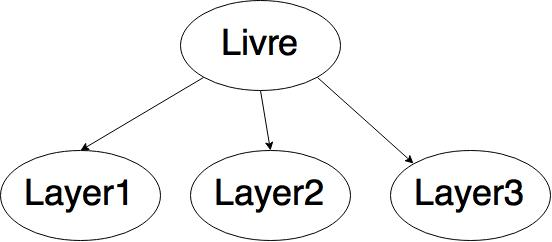
\includegraphics[width=0.25\textwidth]{conception_ezb}
\end{wrapfigure}
\begin{itemize}
    \item un ensemble de layers \footnote{Dans le cadre d'\ezb\ , layer représente la conception de couche où on peux ajouter des citations et résumés} fondé sur un livre
    \item chaque layer devait contenir une liste de citations du texte original et de résumés
\end{itemize}
Avec cette conception, on ne peux pas créer une structure multi-échelles qui permet d'une création de sous-layer d'un layer, qui est intéressant pour faire des commentaires, etc.

La conception était amélioré par Ophir qui a proposé une manière plus adaptable :\textbf{Couches à thème}. Dans cette version, 
\begin{wrapfigure}{r}{0.4\textwidth}
    \centering
    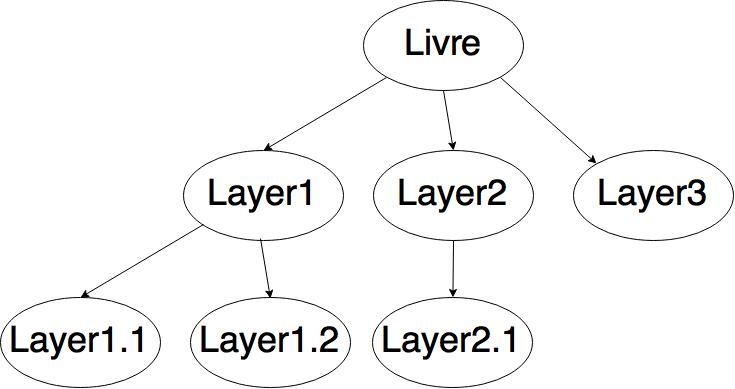
\includegraphics[width=0.4\textwidth]{conception_mini}
\end{wrapfigure}
\begin{itemize}
    \item le livre d'un projet est traité comme un layer
    \item des layers sont fondés sur quelconque layer du projet
    \item chaque layer devait contenir une thème comprenant citation, résumé, traduction, ect
\end{itemize}

\subsection{Analyse des fonctionnelles}
Les changements fonctionnelles d'\mini\ avaient concentré sur les parties des gestions de livres et de projets. 
Les parties des gestions d'utilisateurs et de groups sont bien définies dans \ezb\ , mais pas dans \mini\ .  

\subsubsection{La gestion de livres}
\begin{center}
\begin{tabular}{ |c|c|c| }
\hline
\ezb\ & \mini\ \\ 
\hline
Format ePub                  &  Multi-format \\ 
Gardé comme un fichier .epub &  Gardé dans \db\ en structure \\ 
Non télécharger-able         &  Télécharger-able en multi-format \\
\hline
\end{tabular}
\end{center}

\subsubsection{La gestion de projets}
\begin{center}
\begin{tabular}{ |c|c|c| }
\hline
\ezb\ & \mini\ \\ 
\hline
4 niveaus de finalités à choisir par les utilisateurs \footnotemark & Finalité des paragraphes et des chapitres \\ 
Création de layers du livre & Création de layers des toutes layers \\ 
Citations et résumés & Citation et tous les types de écritures possibles \\
\hline
\end{tabular}
\end{center}
\footnotetext{ Higly Detailed, Fairly Detailed, Fairly Abridged et Highly Abridged } 

\subsubsection{La gestion d'utilisateurs}
Dans \ezb\ , il faut s'inscrire dans le site et tous les utilisateurs sont dans le même niveau de droits qui permet de accéder toutes fonctions fournies par la plate-forme.

\subsubsection{La gestion de groups}
Dans \ezb\ , il y a 3 rôles correspondant différents niveaux de droits de manipuler à choisir quand on ajoute un membre :
\begin{itemize}
    \item \textbf{Owner} qui a tous les droits.
    \item \textbf{Coordinator} qui a le droit d'ajout de membres.
    \item \textbf{Collaborator} qui n'a pas le droit de gérer le groupe.
\end{itemize}

\subsection{Analyse des choix techonologiques}
\begin{center}
\begin{tabular}{|m{5em}|m{5cm}|m{5cm}|}
\hline
& \ezb\ & \mini\ \\ 
\hline
Langage & Scala & JavaScript \\ 
\hline
Database & NoSQL & SQL \\ 
\hline
\end{tabular}
\end{center}